Stochastic reachability games are powerful enough to encode
non-stochastic discounted games~\ref{}. More interestingly, they are
central to the analysis of several important classes of stochastic
games: in particular, stochastic games with parity objectives,
mean-payoff objectives or discounted payoff all reduce to stochastic
reachability games. This motivates the fact that we focused on
reachability for determinacy in~\Cref{6-sec:determinacy}), and that
in~\Cref{6-sec:algos} we only give algorithms for stochastic games
with reachability objectives.


% A schema with the links between non-stochastic MP-discounted-parity
% games and stochastic MP-discounted-parity games, and SSGs.
% 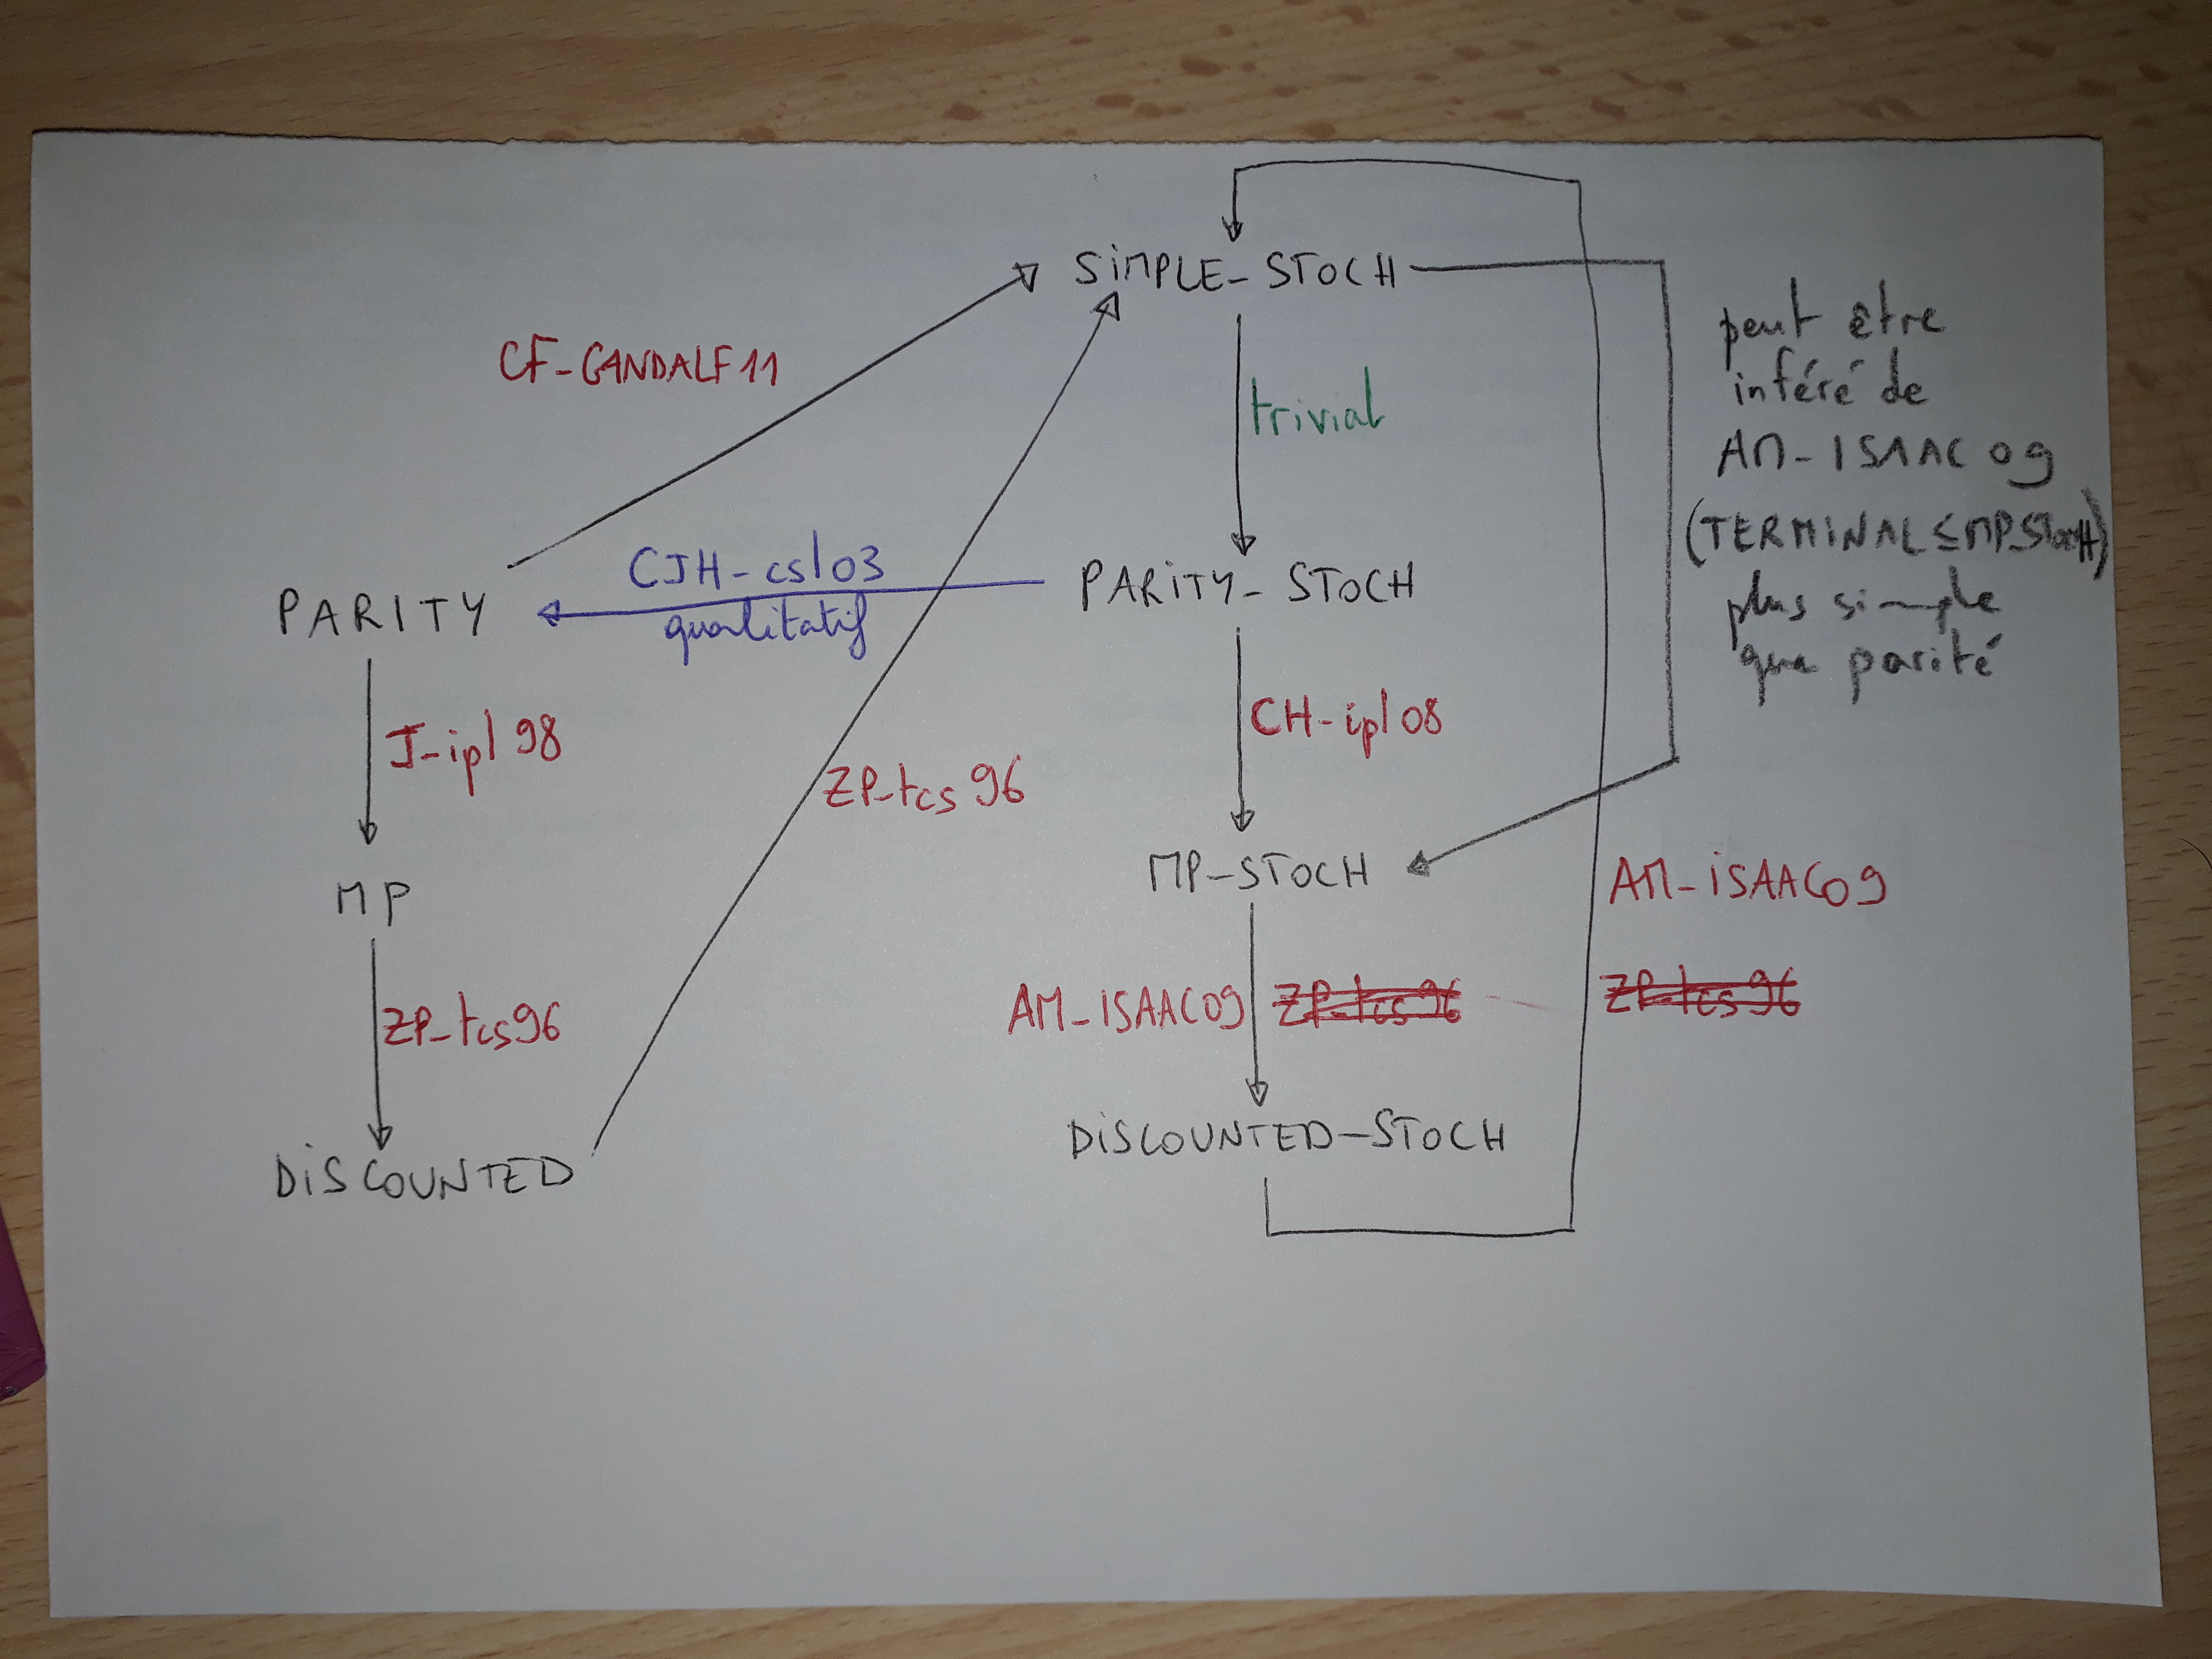
\includegraphics[width=\textwidth]{schema-SSG.jpg}


\subsection{From discounted games to stochastic reachability games}
\nat{reference: ZP-tcs96}

\begin{proposition}
  \label{prop:dg2ssg}
  For any arena $\arena$ with weights in $[0,1]$ and $\lambda$ a
  discount factor, one can construct a stochastic arena $\arena'$ with
  $\Win \subseteq \vertices'$ and an injection
  $\iota : \vertices \to \vertices'$ such that
  $\forall v \in \vertices$
  \[
    \mathsf{value}(v,\arena,\textrm{discount}(\lambda)) =
    \mathsf{value}(\iota(v),\arena',\Reach(\Win)) \enspace.
  \]
\end{proposition}

\begin{proof}
  The idea of the transformation is simple. The vertices in $\arena'$
  are formed of the vertices in $\arena$ plus two sink vertices
  $\smiley$ and $\frownie$, and some fresh random vertices. Then, an
  edge $e = (v,\weight,v')$ of $\arena$ is simulated in $\arena'$ with
  a transition from $v$ to a random vertex $v_e$, and the distribution
  $\delta(v_e)$ assigns probability $\lambda$ to $v'$,
  $(1{-}\lambda)\weight$ to $\smiley$ and $(1{-}\lambda)(1{-}\weight)$
  to $\frownie$. The set $\Win$ of target vertices in $\arena'$
  consists of $\{smiley\}$. To complete the reduction, we let $\iota$
  be the identity function on vertices of $\arena$.

  Note that the transformation from $\arena$ to $\arena'$ is clearly
  polynomial.


  To establish that this transformation preserves the values,
  \emph{i.e.}\ that for every $v \in \vertices$,
  $\mathsf{value}(v,\arena,\textrm{discount}(\lambda)) =
  \mathsf{value}(v,\arena',\Reach(\Win))$, we prove that these
  values are solutions to the same system of equations.

  In the sequel, we write $\mathsf{value}_{\arena'}(v)$ as a shortcut
  for $\mathsf{value}(v,\arena',\Reach(\Win))$.
  By~\Cref{th:determinacy}, the values in the stochastic simple game
  $\arena'$ are solutions to the system of Bellman equations. The sink
  vertices have trivial values, $\mathsf{value}_{\arena'}(\smiley) =1$
  and $\mathsf{value}_{\arena'}(\frownie) =0$.  For every non-random
  vertex $v \notin \{\smiley,\frownie\}$ in $\arena'$,
  \[
    \mathsf{value}_{\arena'}(v)
  = \begin{cases}   \max_{(v,v_e) \in E'}  \mathsf{value}_{\arena'}(v_e) & \text{if}\ v \in \VE \\
     \min_{(v,v_e) \in E'}  \mathsf{value}_{\arena'}(v_e)  & \text{if}\ v \in \VA
   \end{cases}
 \]
 Moreover, for every random vertex $v_e$, with $e=(v,\weight,v')$
 \[
   \mathsf{value}_{\arena'}(v_e) = \lambda \cdot
   \mathsf{value}_{\arena'}(v') + (1{-}\lambda) \weight \cdot
   \mathsf{value}_{\arena'}(\smiley) \enspace.
  \]
 Eliminating the fresh
  random vertices, we obtain that for every non-random vertex
  $v \notin \{\smiley,\frownie\}$ in $\arena'$,
  \[
    \mathsf{value}_{\arena'}(v) =
    \begin{cases}
      \max_{e=(v,\weight,v') \in E}  \lambda \cdot
   \mathsf{value}_{\arena'}(v') + (1{-}\lambda) \weight & \text{if}\ v \in \VE\\
      \min_{(v,\weight,v') \in E}  \lambda \cdot
   \mathsf{value}_{\arena'}(v') + (1{-}\lambda) \weight & \text{if}\ v \in \VA
   \end{cases}
    \]

    We thus observe that the values in $\arena'$, after elimination of
    values for intermediate random vertices, satisfy the equations of
    values in the discounted game (see the proof
    of~\Cref{4-thm:discounted} in~\Cref{chap:4_Payoffs}). Since
    this system of equations has a unique solution, we deduce the
    desired equality:
    $\mathsf{value}_{\arena'}(v) =
    \mathsf{value}(v,\arena,\textrm{discount}(\lambda))$.
    %
    \qed
  \end{proof}

  Remark that~\Cref{prop:dg2ssg} trivially extends to
  discounted stochastic games: from a discounted stochastic game, one
  can build a stochastic reachability game that preserves the values.

\subsection{From stochastic mean-payoff to stochastic discounted}

As a simple generalisation of the non-stochastic case (see
\Cref{4-thm:MP2discounted} \nat{add label to Theorem~4.9}), one can
also provide a reduction from mean-payoff objectives to discounted
payoff objectives, for what concerns stochastic arenas. More
precisely:

\begin{theorem}
  Let $\arena$ be a stochastic arena with integer costs. One can
  effectively compute a discount factor $\lambda^*$ such that for
  every $\lambda \in [\lambda^*,1)$, any optimal pure positional
  strategy profile in the discounted game with discount factor
  $\lambda$ is also an optimal strategy profile in the mean-payoff
  game.
\end{theorem}

\nat{reference AM-isaac'09, Lemmas 1 and 2 (direct proof) + original
  proof without expression for $\lambda^*$ in LL-siamR'69}

\subsection{From stochastic parity  to stochastic mean-payoff}

\nat{reference CH-ipl08, Theorem 3}

\begin{proposition}
  For every stochastic arena $\arena$ with priorities in $[0,d]$, one
  can construct a weight function from $\vertices$ to $\mathbb{Z}$
  such that $\forall v \in \vertices$, if
  $ \mathsf{value}(v,\arena,\textrm{parity}) \notin \{0,1\}$, then
  \[
    \mathsf{value}(v,\arena,\textrm{parity}) =
    \frac 1 2 (\mathsf{value}(v,\arena,\textrm{mean\_payoff})  {+} 1) \enspace.
  \]
\end{proposition}

\begin{proof}
  One can pre-compute the vertices with value $1$ (resp. $0$) for the
  parity objective in polynomial time.
  % ~\cite{} \fbox{ref?}.
  \nat{ref for this ? Florian}
  Let us
  write $W_\Eve$ and $W_\Adam$ for these sets, respectively. We let
  $p_{\min}$ be the minimal probability that appears in the arena
  $\arena$, and $n$ be the number of vertices.
  
  We define the following weight function: for every $v \in W_\Eve$,
  to every edge $(v,k,v')$ in the parity game, we associate the weight
  $1$; for every $v \in W_\Adam$, to every edge $(v,k,v')$, we associate
  the weight $-1$; most importantly, for every
  $v \notin W_\Eve \cup W_\Adam$, to every edge $(v,k,v')$, we associate the
  weight $(-1)^k (2n)^k p_{\min}^{-nk}$.

  Let us prove that the above weight function satisfies
  \[
    \forall v \in \vertices \setminus (W_\Eve \cup W_\Adam),\ 
    \mathsf{value}(v,\arena,\textrm{parity}) = \frac 1 2
    (\mathsf{value}(v,\arena,\textrm{mean\_payoff}) {+} 1)\enspace.
  \]
  To do so, we prove both inequalities.

  \fbox{here we assume sinks for $W_\Eve$ and $W_\Adam$, with
    appropriate priorities}
  
  \begin{lemma} Let $v \in \vertices$. Let $\sigma$ be a pure
    positional optimal strategy for Eve in the parity game
    $(\arena,\textrm{parity})$. For every positional strategy $\tau$
    of Adam
    $\probm_{\sigma,\tau}^v(\Reach(W_\Adam)) \leq 1 -
    \mathsf{value}(v,\arena,\textrm{parity})$.
    \end{lemma}
    This is a direct consequence of the definition of the value.

    \begin{lemma}
      Let $\sigma$ be a pure positional optimal strategy for Eve in
      the parity game $(\arena,\textrm{parity})$. For every positional
      strategy $\tau$ of Adam, for every BSCC $C$ induced by
      $(\sigma,\tau)$ different from $W_\Adam$ and $W_\Eve$,
      $\probm_{\sigma,\tau}^C(\textrm{parity}) >0$.
    \end{lemma}
    \begin{proof}
      Indeed, $\mathsf{value}(C,\arena,\textrm{parity}) \in (0,1)$ by
      definition. Since $\sigma$ is optimal, for $v \in C$,
      $\probm_{\sigma,\tau}^v(\textrm{parity}) \geq
      \mathsf{value}(v,\arena,\textrm{parity}) >0$ (and even
      $\probm_{\sigma,\tau}^v(\textrm{parity})=1$).
    \end{proof}
    As a consequence, the maximum parity in $C$ is even since all
    vertices of $C$ are visited infinitely-often almost-surely when
    starting from $C$ and playing $(\sigma,\tau)$.

    Corollary: under $(\sigma,\tau)$ with $\sigma$ optimal for parity,
    apart from the $W_\Adam$ BSCC, all BSCC are ``good'' for \Eve.

    \begin{lemma}
      Let $\sigma$ be a pure positional optimal strategy for Eve in
      the parity game $(\arena,\textrm{parity})$. For every positional
      strategy $\tau$ of Adam, for every good BSCC $C$ induced by
      $(\sigma,\tau)$, $\MeanPayoff_{\sigma,\tau}^C(\arena) \geq 1$.
    \end{lemma}
    \begin{proof}
      The case $C = W_\Eve$ is trivial. We assume
      $C \cap W_\Eve = \emptyset$ in the sequel.
      
      Let $v$ be a vertex with maximal parity $d_C$ (hence even and
      non-zero) in $C$. Starting from $C$ and under $(\sigma,\tau)$,
      the frequency of $v$ is at least $\frac{1}{n} p_{\min}^n$
      \fbox{to be argued}

      Given the definition of the weight function, the mean-payoff
      from $C$ and under $(\sigma,\tau)$ is at least
      \[
        \frac{1}{n} p_{\min}^n (2n)^{d_C} p_{\min}^{-n d_C} -
        (2n)^{d_C -1} \frac{1}{p_{\min}^{n (d_C-1)}} = (2n)^{d_C -1}
        \frac{1}{p_{\min}^{n (d_C-1)}} =
        (\frac{2n}{p_{\min}^n})^{d_C{-}1}\enspace.
      \]
      Here, we bounded from above the frequency of over states in $C$
      by $1$, and considered the worst case, \emph{i.e.}, parity
      $d_C-1$.
    \end{proof}

    \begin{eqnarray*}
      \MeanPayoff_{\sigma,\tau}^{v} & \geq & - \probm_{\sigma,\tau}^v(\Reach(W_\Adam)) + \sum_{C \textrm{ Good BSCC}} \probm_{\sigma,\tau}^v(\Reach(C))\\
                                    & \geq & -1 + \mathsf{value}(v,\arena,\textrm{parity}) + \probm_{\sigma,\tau}^v(\Parity)\\
                                    & \geq & -1 + \mathsf{value}(v,\arena,\textrm{parity}) + \inf_{\tau'} \probm_{\sigma,\tau'}^v(\Parity)\\
                                    & \geq & -1 + \mathsf{value}(v,\arena,\textrm{parity}) + \mathsf{value}(v,\arena,\textrm{parity})\\
                                    &  \geq & -1 + 2  \mathsf{value}(v,\arena,\textrm{parity}) \enspace.
    \end{eqnarray*}

    Assume again that $\sigma$ is positional optimal for the parity
    objective, and fix $\tau$ an optimal counterstrategy for \Adam in
    $(\arena,\MeanPayoff)$. We deduce:
    \begin{eqnarray*}
      -1 + 2 \mathsf{value}(v,\arena,\textrm{parity}) & \leq & 
                                                               \MeanPayoff_{\sigma,\tau}^{v}\\
                                                      & = & \inf_{\tau'}
                                                            \MeanPayoff_{\sigma,\tau'}^{v}\\
                                                      & \leq &
                                                                \sup_{\sigma'}\inf_{\tau'}
                                                               \MeanPayoff_{\sigma',\tau'}^{v}\\
                                                      & = & 
                                                            \mathsf{value}(v,\arena,\MeanPayoff) \enspace.
    \end{eqnarray*} 
    %
    This proves the first inequality.

    The reverse inequality, can be proved by swapping the roles of
    $\Eve$ and $\Adam$ everywhere.
\end{proof}

Figure~\ref{6-fig:reductions} summarizes the relations between classes
of stochastic games.
